\section{Solving the Program}
\label{sec:methods}

Queue-Haul (Fig.~\ref{fig:sites}) solves the staged program as a short
ordered stack (Fig.~\ref{fig:pipeline}). Each stage is a convex program.
Two implementation details, backend choice and preconditioning, are worth stating
before we turn to the dual structure, which is where the payoff lies.

\begin{figure}[t]
\centering
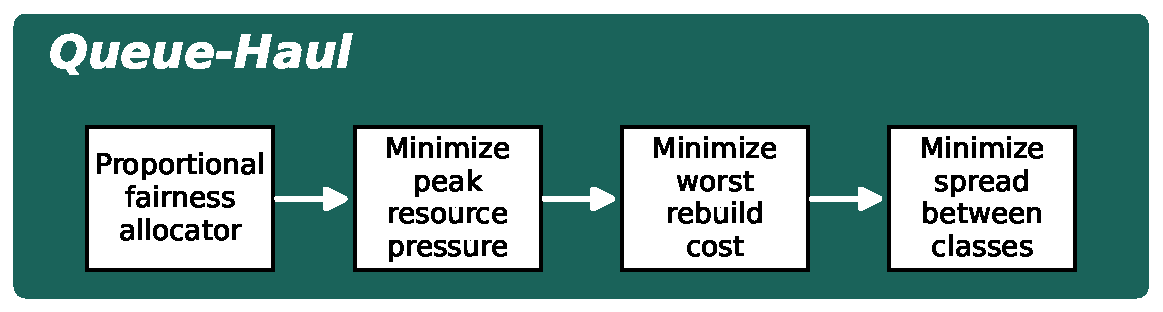
\includegraphics[width=\linewidth]{queue-haul-pipeline.pdf}
\caption{The ordered program Queue-Haul solves (Sec.~\ref{sec:formulation}).
A proportional-fair migration allocator comes first, then refinements that minimize peak
resource pressure, worst-class rebuild cost, and cross-class spread. Each box fixes
the previous one's optimum before optimizing its own objective.}
\label{fig:pipeline}
\end{figure}

\paragraph{Backends.} Stage~1's proportional-fair log-utility
$\sum_q n_q\log(1-z_q/n_q)$ has a gradient that blows up as $z_q\!\to\!0$, so it needs a
conic solver and tight tolerances. We build every stage in
CVXPY~\cite{diamond2016cvxpy}. The pure-LP stages use an LP solver, while
Stage~1 and the Stage-2 tie-breaking QP go to the conic solver Clarabel~\cite{clarabel}.
A loose tolerance on the log-utility lets the iterate drift below the utility floor
and breaks the guarantee handed to later stages.

\paragraph{Preconditioning.} The raw coefficients span about twenty orders of
magnitude. Network terms are bytes
($\beta_q T_q,\,\eta_q T_q\sim10^{8\text{--}11}$), while prefill terms are
GPU-seconds ($T_q/\rho_q\sim10^0$). Left unscaled, this spread wrecks the
conditioning of both the LP and any first-order method. We normalize every capacity
row to $O(1)$. Dividing $L_i\le C_i$ by $C_i$ turns it into $p_i\le1$ with unit
right-hand side, and writes the whole program directly in the pressures $p_i$ it
already uses. This one rescaling is also what makes the first-order methods below tractable.

\paragraph{Ordered-problem linking.} Each stage re-solves the full program with the
earlier optima as a constraint. Stage 2 adds the fairness floor $U(z)\ge U^\star-\delta$, Stage 3 adds
that plus $p_i\le\phi^\star$ for all $i$, and so on.

\subsection{Resource-pressure and its dual}
Stage 2 is where the meaning of duality is richest in our problem, because its peak-pressure objective turns
the multipliers into congestion prices. We dualize the pressure ceilings
$p_i(x)\le\phi$ with multipliers $\pi_i\ge0$. The Lagrangian is
$\phi\big(1-\sum_i\pi_i\big)+\sum_i\pi_i\,p_i(x)$, so minimizing over the free
$\phi$ forces
\[
\sum_{i\in\mathcal{I}}\pi_i=1.
\]
With $\phi$ gone the inner problem is linear in $x$
and \emph{separates by class}. Each class sends its $n_q$ jobs to whichever
$(\ell,a)$ is cheapest at the current prices,
\[
\begin{aligned}
\mathrm{cost}^R_{q\ell}(\pi)&=\pi^{\mathrm{net}}_\ell\tfrac{\beta_q T_q}{C^{\mathrm{net}}_\ell}+\pi^{\mathrm{pfill}}_{\ell m}\tfrac{T_q/\rho_q}{C^{\mathrm{pfill}}_{\ell m}},\\
\mathrm{cost}^S_{q\ell}(\pi)&=\pi^{\mathrm{net}}_\ell\tfrac{\eta_q T_q}{C^{\mathrm{net}}_\ell}+\pi^{\mathrm{ing}}_{\ell m}\tfrac{\eta_q T_q}{C^{\mathrm{ing}}_{\ell m}}.
\end{aligned}
\]
So $\pi_i$ is the marginal congestion price of resource $i$, or how much the peak
moves if that resource is throttled. CVXPY returns these prices exactly as the
ceiling duals, and they are interpretable on their own, naming which resource
binds and by how much.

\paragraph{An envelope-theorem check.} The prices also predict sensitivity. Every
capacity is linear in the deadline, $C_i\propto D$, so the envelope identity
$\partial\phi^\star/\partial\ln C_i=-\pi_i\hat p_i$ composes to
\[
\frac{d\phi^\star}{dD}=-\frac{1}{D}\sum_{i\in\mathcal{I}}\pi_i\,\hat p_i,
\]
with $\hat p_i$ the realized pressures. Both predictions are testable from a single LP solve.
Table~\ref{tab:sens} reports these per-resource sensitivities for the base instance
and confirms each against a $1\%$ finite-difference perturbation.

\subsection{First-order methods for the dual}

The per-class separation lends itself to ascending the dual of Stage 2 instead of calling a
general LP solver. Two prices drive it, namely $\pi$ on the resource ceilings (confined to
the simplex $\sum_i\pi_i=1$) and $\nu\ge0$ on the proportional-fair floor
$U(z)\ge U^\star-\delta$. The dual function is
\[
g(\pi,\nu)=\nu(U^\star-\delta)+\min_{x,z\ge0}\Big[\sum_i\pi_i\,p_i(x)-\nu\,U(z)\Big],
\]
which we maximize. Each evaluation is cheap and separable. Every class routes its
$n_q$ jobs to the cheapest $(\ell,a)$ at prices $\pi$, weighing migration against the
proportional-fair penalty $-\nu\,n_q\log(1-z_q/n_q)$ on whatever it strands.

\smallskip\noindent\textbf{Projected subgradient.} Step uphill, then project $\pi$
back onto the simplex and clip $\nu$ at zero,
\begin{align}
\pi^{k+1}&=\Pi_\Delta\!\big(\pi^k+s_k\,\hat p^k\big),\\
\nu^{k+1}&=\big(\nu^k+s_k\,[(U^\star-\delta)-U(\hat z^k)]\big)_+,
\end{align}
with a Polyak step $s_k=(\phi^\star-g^k)/\|\hat g^k\|^2$ off the known optimum.

\smallskip\noindent\textbf{Mirror descent.} We swap the Euclidean projection
for a multiplicative, exponentiated-gradient step~\cite{beck2003mirror}, which
respects the simplex geometry and better matches the $\ell_\infty$ peak,
\[
\pi_i^{k+1}\propto\pi_i^k\exp\!\big(s_k\,\hat p_i^k\big),\quad\text{renormalized},
\]
with $\nu$ stepped as above. The per-iteration cost is the same, with better constants and geometry.

\smallskip\noindent\textbf{ADMM.} We give each class a private assignment
and a consensus copy $\bar p$ of the per-resource loads, then
alternate three updates~\cite{boyd2011admm}. A per-class QP routes or strands each class
under the fairness penalty plus a quadratic pull toward $\bar p$. A prox-of-max
reads the peak $\phi$ off the pooled loads. A dual ascent then corrects wherever the assignments and the consensus disagree.

\begin{figure}[t]
\centering
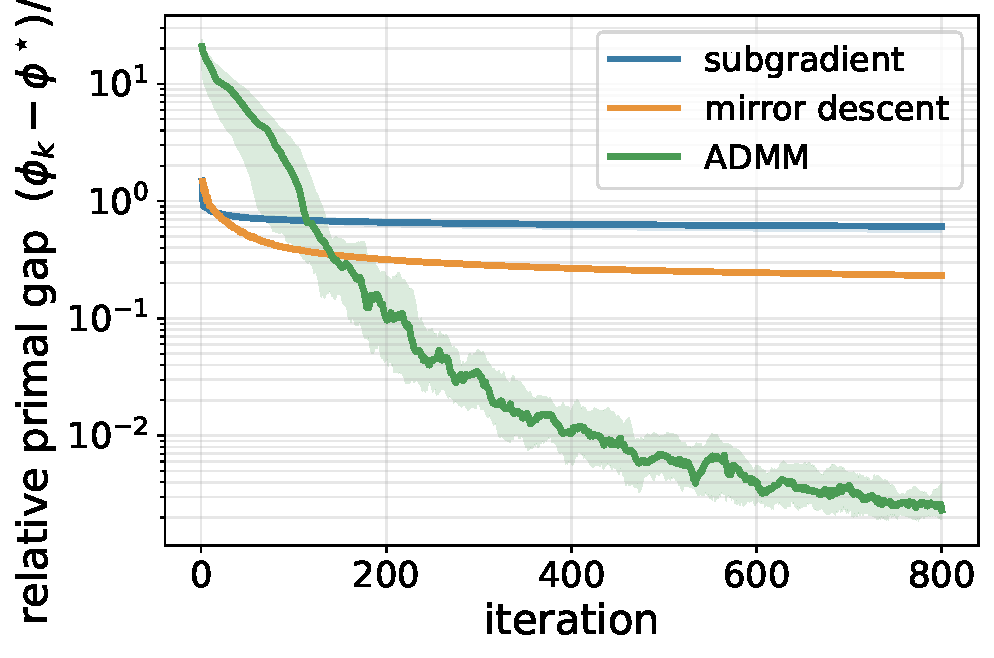
\includegraphics[width=\columnwidth]{stage2_convergence.pdf}
\caption{First-order dual solvers converging to the CVXPY optimum (median and 25--75\%
band over $50$ random instances, $L=3$). The gradient methods plateau far from
$\phi^\star$, mirror descent leading subgradient as the simplex geometry predicts.
ADMM costs a per-class QP each step, but over the full budget it overtakes both near
iteration $120$ and drives the gap to ${\sim}2\times10^{-3}$.}
\label{fig:convergence}
\end{figure}

Figure~\ref{fig:convergence} splits the three in two. The gradient methods plateau.
At $800$ iterations the median relative gap to $\phi^\star$ is $0.60$ (subgradient)
and $0.23$ (mirror descent), mirror ahead just as the simplex geometry predicts.
ADMM starts worst, but over the full budget it overtakes both near iteration $120$
and drives the gap to $2\times10^{-3}$. So the one method that truly converges is the
one that pays a QP per step. The gradient methods stall for three reasons. The peak
is non-smooth, so the subgradient is a single active constraint and the iterate
chatters. The step starves when the fairness floor is slack and $\nu$ rests at zero.
And one global step size fits the per-class prices poorly. ADMM sidesteps all three
by solving each class exactly. For exact solves we still lean on CVXPY, but ADMM is
the clear direction to build on.

